\documentclass{article}
\usepackage{placeins}
\usepackage{array}
\usepackage{float} 
\usepackage{graphicx} % Required for inserting images

\title{Daylighting with skylights in different climates: creating cost saving comfortable infrastructure.}
\author{Samara Elling}
\date{July 2026}

\begin{document}

\maketitle

\section{Introduction}

    This paper outlines the process of comparing the climate of Mount Angel, Oregon and Santa Fe, New Mexico, and modifying a daylighting skylight design specific to Mount Angel's climate to be able to be used in Santa Fe's climate. This also creates a basis for other areas hoping to use similar daylighting strategies in other climates. The original model uses a combination of light reflectors and light regulators to control and keep the levels of light in a room within a certain comfortable range. It is designed to work in a wide range of  light conditions while spreading the light evenly around the room with little variation. It is meant for certain rooms such as classrooms that are in operation between 9 am to 5 pm. This is meant to eliminate the need for electric lighting during most working hours, saving electricity and energy. 


\section{Goals}


The original designs were meant for a classroom in the new buildings of mount angel Abby business center in  Oregon, it's designed to provide comfortable light between schooling hours which are 9 am - 5 pm. The criteria of comfortable lighting was set to 20-45 foot candles which is enough to take notes, type, and for general office activities. The design achieved this incredibly well with the room being evenly lit in that range around 95 percent of the outlined time in the entire year. This completely eliminated the need for electric lights in the classroom leading the collage to forgo all electric lighting in the classrooms with the skylight. This type of design was implemented in seven classrooms in the building with the same effectiveness, saving electric energy as well as providing a more comfortable experience then most artificial lighting. If implemented in classrooms the average saved energy per classroom would be anywhere from 9,000 to 10,000 kilowatt-hours which can cost 1,700 to 1,900 US dollars per classroom per year. 

\section{System Design}

The skylight distributes light by combining louvers and reflectors suspended below the opening with a 16in gap to allow light through the middle. The reflectors consist of opaque aluminum prisms that reflect 95 percent of incident light due to a custom white reflective glaze. the reflectors are arranged in three sections of graduating density and cover about 16 percent of the rooms floor area to distribute the light evenly throughout the room even the sides and corners. The reflectors allow the light to be consistently distributed in the room no matter the conditions outside while the louvers account for keeping the light within the range of 20 - 45 foot candles (fc's). The louvers rotate in increments of five degrees, they run on a program designed to measure the outside light and open to let in certain amounts of available light and self adjust to keep the room within the range of 20-45 fc's. When they are completely open they let in 72 percent of the light having an average daylight factor of 3.8 and when they are fully closed they let in 6 percent with an average daylight factor of 0.3 , this range allows them to be effective in nearly all conditions of light. The louver system is controlled by a switch that opens the louvers when flipped, acting like a light switch. 

\begin{figure}[!htb]
    \centering
    \includegraphics[width=0.5\linewidth]{reflectorslayout.png}
    \caption{Graduating Reflectors Design}
    \label{fig:placeholder}
\end{figure}
\section{Process}

for this project the same dimension of the room 30ft x 30ft as the Mount Angel classroom was used because of the lack of classroom to model it after in Santa Fe and used existing studies of the skylight system in order to be as accurate as possible without the physical equipment and models needed to be completely accurate. 

To create the design I tried to understand the way that the reflectors and skylight diffused light. I created light studies with each component of the reflection system with the maximum light level for Santa Fe. I made diagrams and studied the way light would bounce off of each of the components. The result of just a skylight was a central bright spot the room, and with only the louvers it was more concentrated around the center with less dispersion. I made charts of the foot candles whin the room by mapping a 2ft by 2ft grid of the dimensions and putting the average foot candles for each section in each grid. To fully understand the way light would be distributed regardless of the light available in the sky we created a similar chart of the daylight factor of each grid. this is to allow estimations of the illumination based on the foot candles available outside without calculating each individual condition. The formula for calculating daylight factors;

\begin{equation}
    $$ Daylight Factor = Indoor lllumination(FC) / outside illumination(FC) * 100 $$
\end{equation}

A daylight factor is the percentage of the light from outside that makes it to a given area inside 

With only the reflectors the light was brighter around a ring around the skylight with it being dimmer around the edges and middle. With both the reflectors and the louvers the light was evenly dispersed and a bit dimmer. In all the trials, the light levels in the room were around 100 or more foot candles too high when calculated with Santa Fe light levels. In order to solve this I researched the differences between Mount Angel and Santa Fe to find the cause. The main differences that could affect it are the solar altitude or sun angle differences,  the solar radiation levels, and the altitude, all of which affect the illumination or heat transfer into the room. 


The first thing examined was the solar altitude and how it affects the light. In Oregon, the maximum solar altitude is around 70 degrees while the maximum in Santa Fe is around 80 degrees. Mount angel has a smaller minimum solar altitude then Santa Fe with a minimum of 21 degrees while Santa Fe has a minimum of 30 (sun, wind, and light). This is due to the difference in latitude of both city's which affects the angle of the sun coming through the skylight which changes the way the light is distributed in the room, with more direct bright spots. This comes from the way light is hitting surfaces, with steeper angles its more direct and brighter, it also affects the undertone colors, shallow angles produce cooler undertones while direct angles produce more red and yellow light.  To combat this, the angle that the skylight is situated was changed to be 70 degrees facing north in order to only take in indirect sunlight to get less light. 

\begin{figure}[!htb]
    \centering
    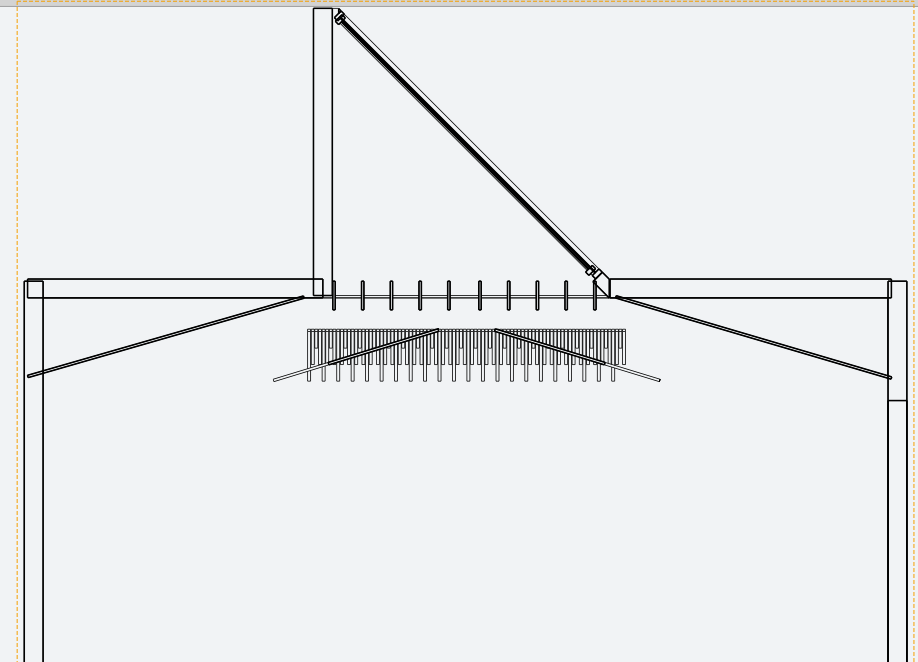
\includegraphics[width=0.9\linewidth]{archetecturesegment.png}
    \caption{first modification}
    \label{fig:placeholder}
\end{figure}
\FloatBarrier

At first, the light levels for the latitude reported in the book "Sun, Wind, and Light" weren't consistent with the light reported from the Santa Fe airport and local colleges. after investigation it was found that the elevation was not taken into account and the illumination levels that were taken from the book Sun, Wind, and Light which were measurements from Phoenix, Arizona which is on a similar latitude but much different altitudes . This led the first set of calculations to be wrong because they were done with less light levels than is reality in Santa Fe. After realizing the inconsistency and what caused it the information for the future calculations are from Santa Fe regional airport reports and collage measurements to get more accurate information. 

The difference in elevation is about 6,800 ft affecting illumination, because less atmosphere is between the sunlight and the ground meaning theirs less to disperse and diffuse the light making it brighter by about 20-45 percent  depending on the place and conditions. After the modification and the correction I made light study diagrams and light charts to see the effectiveness of the modification. In this case there was still  more than double the amount of light aimed for in the room. I went through a couple of variations to fix this, the first was increasing the density of the reflectors to reflect less of the light around the room. However that wasn't effective enough, the second variation was decreasing the reflectivity of the reflectors in order to have less of the light that makes it through the skylight get distributed around the room which was also too little.  Which Because of this the area of the skylight was lessened in order to receive less light, originally it was around 100 square ft which was reduced to 80 based on a ratio of the average illumination in Mount Angel to Santa Fe.  The amount of transmission  that the Mount Angel skylight received was about 72 percent of the light available in the sky with the original design, to find the right amount to reduce the surface area by we found how much Santa Fe would need to receive by calculating a daylight factor target and rationing it with the amount of light available. Santa Fe needs about 58 percent transmission compared to 72 percent leading to the reduction of the surface area by 20 percent. This kept the light in the correct range even at the brightest illumination outside, 12,100 foot candles. 
\begin{table}[ht]
\centering
\caption{final design light study}
% This shrinks the massive table to fit exactly within the text margins:
\resizebox{\linewidth}{!}{
    % The 13 'c's separated by '|' create the 13 columns with vertical gridlines
    \begin{tabular}{|c|c|c|c|c|c|c|c|c|c|c|c|c|}
    \hline
    29 & 31.1 & 34 & 35.5 & 37.7 & 39.1 & 39.9 & 39.1 & 37.7 & 35.5 & 34 & 31.1 & 29 \\ \hline
    31.1 & 33.3 & 35.5 & 37 & 37.7 & 38.4 & 38.4 & 38.4 & 37.7 & 37 & 35.5 & 33.3 & 31.1 \\ \hline
    34 & 35.5 & 37.7 & 37.7 & 37.7 & 37.7 & 37.7 & 37.7 & 37.7 & 37.7 & 37.7 & 35.5 & 34 \\ \hline
    36.3 & 37.7 & 38.4 & 36.2 & 33.3 & 35.5 & 37.7 & 35.5 & 33.3 & 36.2 & 38.4 & 37.7 & 36.3 \\ \hline
    39.1 & 39.1 & 39.1 & 34.8 & 29.7 & 34 & 38.4 & 34 & 29.7 & 34.8 & 39.1 & 39.1 & 39.1 \\ \hline
    40.6 & 40.6 & 39.9 & 35.5 & 31.1 & 34.8 & 38.4 & 34.8 & 31.1 & 35.5 & 39.9 & 40.6 & 40.6 \\ \hline
    42.8 & 41.3 & 40.6 & 37 & 32.6 & 36.2 & 39.1 & 36.2 & 32.6 & 37 & 40.6 & 41.3 & 42.8 \\ \hline
    40.6 & 40.6 & 39.9 & 35.5 & 31.1 & 34.8 & 38.4 & 34.8 & 31.1 & 35.5 & 39.9 & 40.6 & 40.6 \\ \hline
    39.1 & 39.1 & 39.1 & 34.8 & 29.7 & 34 & 38.4 & 34 & 29.7 & 34.8 & 39.1 & 39.1 & 39.1 \\ \hline
    36.3 & 37.7 & 38.4 & 36.2 & 33.3 & 35.5 & 37.7 & 35.5 & 33.3 & 36.2 & 38.4 & 37.7 & 36.3 \\ \hline
    34 & 35.5 & 37.7 & 37.7 & 37.7 & 37.7 & 37.7 & 37.7 & 37.7 & 37.7 & 37.7 & 35.5 & 34 \\ \hline
    31.1 & 33.3 & 35.5 & 37 & 37.7 & 38.4 & 38.4 & 38.4 & 37.7 & 37 & 35.5 & 33.3 & 31.1 \\ \hline
    29 & 31.1 & 34 & 35.5 & 37.7 & 39.1 & 39.9 & 39.1 & 37.7 & 35.5 & 34 & 31.1 & 29 \\ \hline
    \end{tabular}
}

\textbf{each square is 2ftx2ft of the room\\
louvers completely closed\\
12,077 foot candles available\\
average inside FC; 36.5\\
average DF; 0.3}

\end{table}

\section{Results}

The final design is a 70 degree steep 8 ft by 10 ft north facing skylight with louvers and reflectors that transmits 58 percent of all light available  in the sky into the room. By modifying it like this the daylight factor in the room is consistently averaged 3.8 percent with the louvers all the way open and 0.3 percent with the louvers all the way closed. This allowed the room to say within the desired range of 20- 45 foot candles even on the brightest days with nearly 12,100 foot candles in the sky and stay in the same range when theirs only 500 fc's. In other climates the design should consist of a similar reflector set that replicates the properties of the original in different materials or styles. Materials such as glass, fabric, and panels could be used to replicate the attributes of the original designs. The skylight reflectors should span 16 percent of the room from the center opening with a 16in gap to the skylight for the best results. The skylight itself should be tilted north(south in the southern hemisphere or in very dim climates) in order to control the intensity of light coming in at an angle slightly less then the maximum solar altitude of the location. 

\begin{figure}[!htb]
    \centering
    \includegraphics[width=0.9\linewidth]{finalsectionview.png}
    \caption{final design}
    \label{fig:placeholder}
\end{figure}

\section{Sources }

\begin{itemize}
    \item Sun, Wind, and Light; Architectural Design Strategies, Third edition. MARK DeKAY and G. Z. BROWN. 
    \item The Passive Solar Energy Book. Edward Mazria
    \item Energy Studies, University of Oregon
    \item https://www.velux.com/healthy-buildings/research-and-knowledge/deic-basic-book/daylight/daylight-calculations-and-measurements 
    \item https://www.timeanddate.com/sun/usa/santa-fe
    \item https://www.healio.com/news/ophthalmology/20120331/the-physics-of-light 
\end{itemize}

\end{document}
